%%%%%%%%%%%%%%%%%%%%%%%%%%%%%%%%%%%%%%%%%
% Simple Sectioned Essay Template
% LaTeX Template
%
% This template has been downloaded from:
% http://www.latextemplates.com
%
% Note:
% The \lipsum[#] commands throughout this template generate dummy text
% to fill the template out. These commands should all be removed when 
% writing essay content.
%%%%%%%%%%%%%%%%%%%%%%%%%%%%%%%%%%%%%%%%%

%----------------------------------------------------------------------------------------
%	PACKAGES AND OTHER DOCUMENT CONFIGURATIONS
%----------------------------------------------------------------------------------------

\documentclass[12pt]{book} % Default font size is 12pt, it can be changed here
		\textheight = 28cm
		\textwidth = 19cm
		\topmargin = -1cm
		\oddsidemargin = -1cm
		\parindent = 5mm

\usepackage{geometry} % Required to change the page size to A4
\geometry{a4paper} % Set the page size to be A4 as opposed to the default US Letter

\usepackage{graphicx} % Required for including pictures

\usepackage{float} % Allows putting an [H] in \begin{figure} to specify the exact location of the figure
\usepackage{wrapfig} % Allows in-line images such as the example fish picture

%\usepackage{lipsum} % Used for inserting dummy 'Lorem ipsum' text into the template

\linespread{1.1} % Line spacing

%\setlength\parindent{0pt} % Uncomment to remove all indentation from paragraphs
\usepackage[utf8]{inputenc}
\usepackage[spanish]{babel}
\usepackage[T1]{fontenc}
\usepackage{fancyhdr}
\usepackage{multicol}
\usepackage{cite} % para contraer referencias
% Configurar los encabezados, pies de pagina y paginas de capitulo
% Encabezados
\lhead[\thepage]{CAPÍTULO \thechapter. \rightmark}
\chead[]{}
\rhead[CAPÍTULO \thechapter. \leftmark]{\thepage}

\renewcommand{\headrulewidth}{0.5pt}

% Pie de pagina

\lfoot[]{\today}
\cfoot[]{}
\rfoot[J.Carlos Ávila]{}
\renewcommand{\footrulewidth}{0pt}

\usepackage{savesym}
\usepackage{amsmath}
\savesymbol{iint}
\usepackage{txfonts}
\restoresymbol{TXF}{iint}


\usepackage[x11names,table]{xcolor}
\usepackage{pstricks}
\usepackage[colorinlistoftodos, textwidth=2cm, shadow]{todonotes}
%\usepackage{hyperref}



\usepackage[colorlinks]{hyperref}
\usepackage[nogroupskip,nopostdot]{glossaries}
\setglossarystyle{altlist}
\makenoidxglossaries




%\usepackage[toc,style=altlistgroup,hyperfirst=false]{glossaries}


\hypersetup{
    colorlinks=true,
    linkcolor=rosa1,
    filecolor=magenta,      
    urlcolor=cyan,
}

\urlstyle{same}

\graphicspath{{./images/}} % Specifies the directory where pictures are stored

\definecolor{miorange}{rgb}{0.11, 0.43, 0.21}
\definecolor{rosa1}{RGB}{236, 46, 80}

%%%%%%%%%%%%%%%%%%%%%%%%%%%%%%%%%%%%%%%%%%%%%%%%%%%%%%%%%%%%%%%%%%%%%%%%%%%%%%%%%%%%%%%%%%%%%%%%%%%%%%%%%%%
%----------------------------------------------------------------------------------------
%	begin {Glosario}
%----------------------------------------------------------------------------------------

\newglossaryentry{SO}{name={SO},description={Es el sistema o conjunto de aplicaciones que permiten que una computadora lleven a cabo sus funciones.}}
\newglossaryentry{Linux}{name={Linux},description={GNU/Linux Sistema Operativo creado y distribuido por miles de 
													personas alrededor del mundo}}
													
\newglossaryentry{Windows}{name={Windows},description={Sistema Operativo creado y distribuido por Microsoft.}}

\newglossaryentry{Mac}{name={Mac},description={Sistema Operativo creado y distribuido por Apple}}

%%%%%%%%%%%%%%%%%%%%%%%%%%%%%%%%%%%%%%%%%%%%%%%%  %%%%%%%%%%%%%%%%%%%%%%%%%%%%%%%%%%%%%%%%%%%%%%%%%%%%%%%%%
\newglossaryentry{}{name={},description={}}
%%%%%%%%%%%%%%%%%%%%%%%%%%%%%%%%%%%%%%%%%%%%%%%%  %%%%%%%%%%%%%%%%%%%%%%%%%%%%%%%%%%%%%%%%%%%%%%%%%%%%%%%%%

%----------------------------------------------------------------------------------------
%	End {Glosario}
%----------------------------------------------------------------------------------------


\pagestyle{fancy}

\begin{document}

\lhead[\thepage]{CAPÍTULO \thechapter. \rightmark}
\rhead[CAPÍTULO \thechapter. \leftmark]{\thepage}


%----------------------------------------------------------------------------------------
%	TITLE PAGE
%----------------------------------------------------------------------------------------

\begin{titlepage}

\newcommand{\HRule}{\rule{\linewidth}{0.5mm}} % Defines a new command for the horizontal lines, change thickness here

\center % Center everything on the page
 
%----------------------------------------------------------------------------------------
%	HEADING SECTIONS
%----------------------------------------------------------------------------------------

\textsc{\LARGE Instituto Tecnológico de San Juan del Río}\\[1.5cm] % Name of your university/college
\textsc{\Large Centro de Investigación en ciencia Aplicada y Tecnología Avanzada}\\[0.5cm] % Major heading such as course name
%\textsc{\large Minor Heading}\\[0.5cm] % Minor heading such as course title

%----------------------------------------------------------------------------------------
%	TITLE SECTION
%----------------------------------------------------------------------------------------

\HRule \\[0.4cm]
{ \huge \bfseries Amplificación interactiva de contenido por medio de la detección de la dirección de la mirada.}\\[0.4cm] % Title of your document
\HRule \\[1.5cm]
 
%----------------------------------------------------------------------------------------
%	AUTHOR SECTION
%----------------------------------------------------------------------------------------

\begin{minipage}{0.4\textwidth}
\begin{flushleft} \large
\emph{Autor:}\\
J. Carlos \textsc{\'Avila Resendiz} % Your name
\end{flushleft}
\end{minipage}
~
\begin{minipage}{0.4\textwidth}
\begin{flushright} \large
\emph{Supervisor:} \\
Dr. Joaquin  \textsc{Salas Rodriguez} % Supervisor's Name
\end{flushright}
\end{minipage}\\[4cm]

% If you don't want a supervisor, uncomment the two lines below and remove the section above
%\Large \emph{Author:}\\
%John \textsc{Smith}\\[3cm] % Your name


%----------------------------------------------------------------------------------------
%	DATE SECTION
%----------------------------------------------------------------------------------------

{\large \today}\\[1cm] % Date, change the \today to a set date if you want to be precise

%----------------------------------------------------------------------------------------
%	LOGO SECTION
%----------------------------------------------------------------------------------------


\includegraphics{./imagenes/itsjr_s.jpg}\\ % Include a department/university logo - this will require the graphicx package

 
%----------------------------------------------------------------------------------------

\vfill % Fill the rest of the page with whitespace
\newpage
$\ $
\thispagestyle{empty}
\end{titlepage}

%----------------------------------------------------------------------------------------
%	TABLE OF CONTENTS
%----------------------------------------------------------------------------------------j
\setcounter{tocdepth}{3}   %control deptness index
%\setcounter{lofdepth}{2}  % control table of figures depth 
\pagenumbering{roman} 
\tableofcontents % Include a table of contents

\newpage % Begins the essay on a new page instead of on the same page as the table of contents
\thispagestyle{empty} 
%\appendix
%----------------------------------------------------------------------------------------
%	INTRODUCTION
%----------------------------------------------------------------------------------------
\pagenumbering{arabic}	
%\setcounter{page}{1}
	
			 
\newpage		 
\pagestyle{fancy}

%\chapter*{Introducción}
%&\addcontentsline{toc}{chapter}{Introducción}
%	El presente documento expone las principales pautas en el desarrollo de un sistema de asistencia para débiles visuales,

	
	
	



\newpage

\chapter{GENERALIDADES}
\thispagestyle{empty}
\markboth{GENERALIDADES}{GENERALIDADES}

\begin{minipage}{0.5\textwidth}
	\begin{flushleft} \large
	%\emph{•} \\
	\scriptsize	\textsl{\large “El auténtico genio consiste en la capacidad para evaluar información incierta, 
								aleatoria y contradictoria.”}\\
	\scriptsize \textbf{Winston Churchill, estadista.}
	\end{flushleft}
\end{minipage}\\[4cm]			

\newpage
\section{Objetivos}
	\subsection{Objetivo general}
	
		Desarrollar una aplicación de amplificación interactiva para computadoras con sistema operativo Windows, 
		que asista a personas con bajas capacidades visuales, por medio del seguimiento y estimación de la dirección 
		de la mirada sobre la pantalla de la computadora y en base a ello amplificar la zona de la pantalla en la 
		que enfoca la vista.
	
	\subsection{Objetivos específicos}
		\begin{itemize}
			\item Detección precisa y confiable del movimiento del globo ocular, con la ayuda de software de 
			procesamiento de imágenes digitales.
			\item Hacer uso de las API’s del sistema operativo que proveen las herramientas que magnifican la zona de
			la pantalla seleccionada.
			\item Integrar los dos componentes anteriores y de esa forma obtener un magnificador con interacción visual.
			\item Una vez se cuente con un prototipo, realizar pruebas de campo.
		\end{itemize}
		

\newpage
\section{Justificación}
	Pese al avance desmesurado de la tecnología en los últimos años en donde las capacidades de los dispositivos se
	duplica cada cierto tiempo, respondiendo de forma bastante precisa la emblemática ley de 
	\href{https://en.wikipedia.org/wiki/Moore's_law}{Moore} hay aun a día de hoy
	ciertas cuestiones que no han sido abordadas, quizá en gran parte debido al amplio panorama de problemas que se
	pueden afrontar con soluciones tecnológicas y de alguna forma ayudar a solventar o/y hacer más fácil las mismas.
	
	Aun si los programas de asistencia a personas con capacidades diferentes están a día de hoy cobrando mayor 			  	
	relevancia en prácticamente todos los aspectos sociales, pues en la actualidad las posibilidades de llevar una vida
	productiva y sin las limitaciones de antaño, son ya una realidad, entre las herramientas que se proporcionan a este
	sector de la población están las llamadas tecnologías de asistencia o accesibilidad en entornos informáticos, mismas
	que van desde iconos monocromáticos de un mayor tamaño, hasta lectores de pantalla y lupas, siendo estas últimas el
	principal componente proporcionado por las herramientas de accesibilidad de los Sistemas Operativos \gls{SO} actuales,
	siendo común en los tres mas importantes \gls{Linux}, \gls{Windows}, \gls{Mac}.
	
	Siendo de los tres el segundo, Windows, en el cual se enfocaran los esfuerzos de hacer converger las herramientas de
	accesibilidad ya mencionadas y las tecnologías de visión por computadora CV, para ofrecer a los discapacitados 
	visuales una forma de hacer uso de la tecnología, mismos que según datos de la OMS de 2002, eran mas de 161 millones
	de personas, en especifico de computadoras, sin que su limitante visual les impida el poder interactuar con el 
	equipo.
	
	Específicamente el segmento de la población con discapacidad visual en el que se enfoca el desarrollo de este
	proyecto es el de personas que cuentan con cierto grado de visión, o lo que se conoce como resto visual, pues,
	siempre que exista un resto visual por mínimo que sea se debe potenciar su uso para alcanzar el máximo desarrollo
	posible

\newpage 
\section{Caracterización de la empresa}
	\subsection{Datos generales de la empresa}
	\begin{description}
		\item[Nombre de la organización:] Centro de Investigación en Ciencia Aplicada y Tecnología Avanzada del
			 Instituto Politécnico Nacional \texttt{CICATA}
			 
		\item[Dirección:] Querétaro, Cerro Blanco No.141 Col. Colinas del Cimatario, C.P. 76090, Querétaro, Querétaro
			 México.
			 \begin{center}
			 	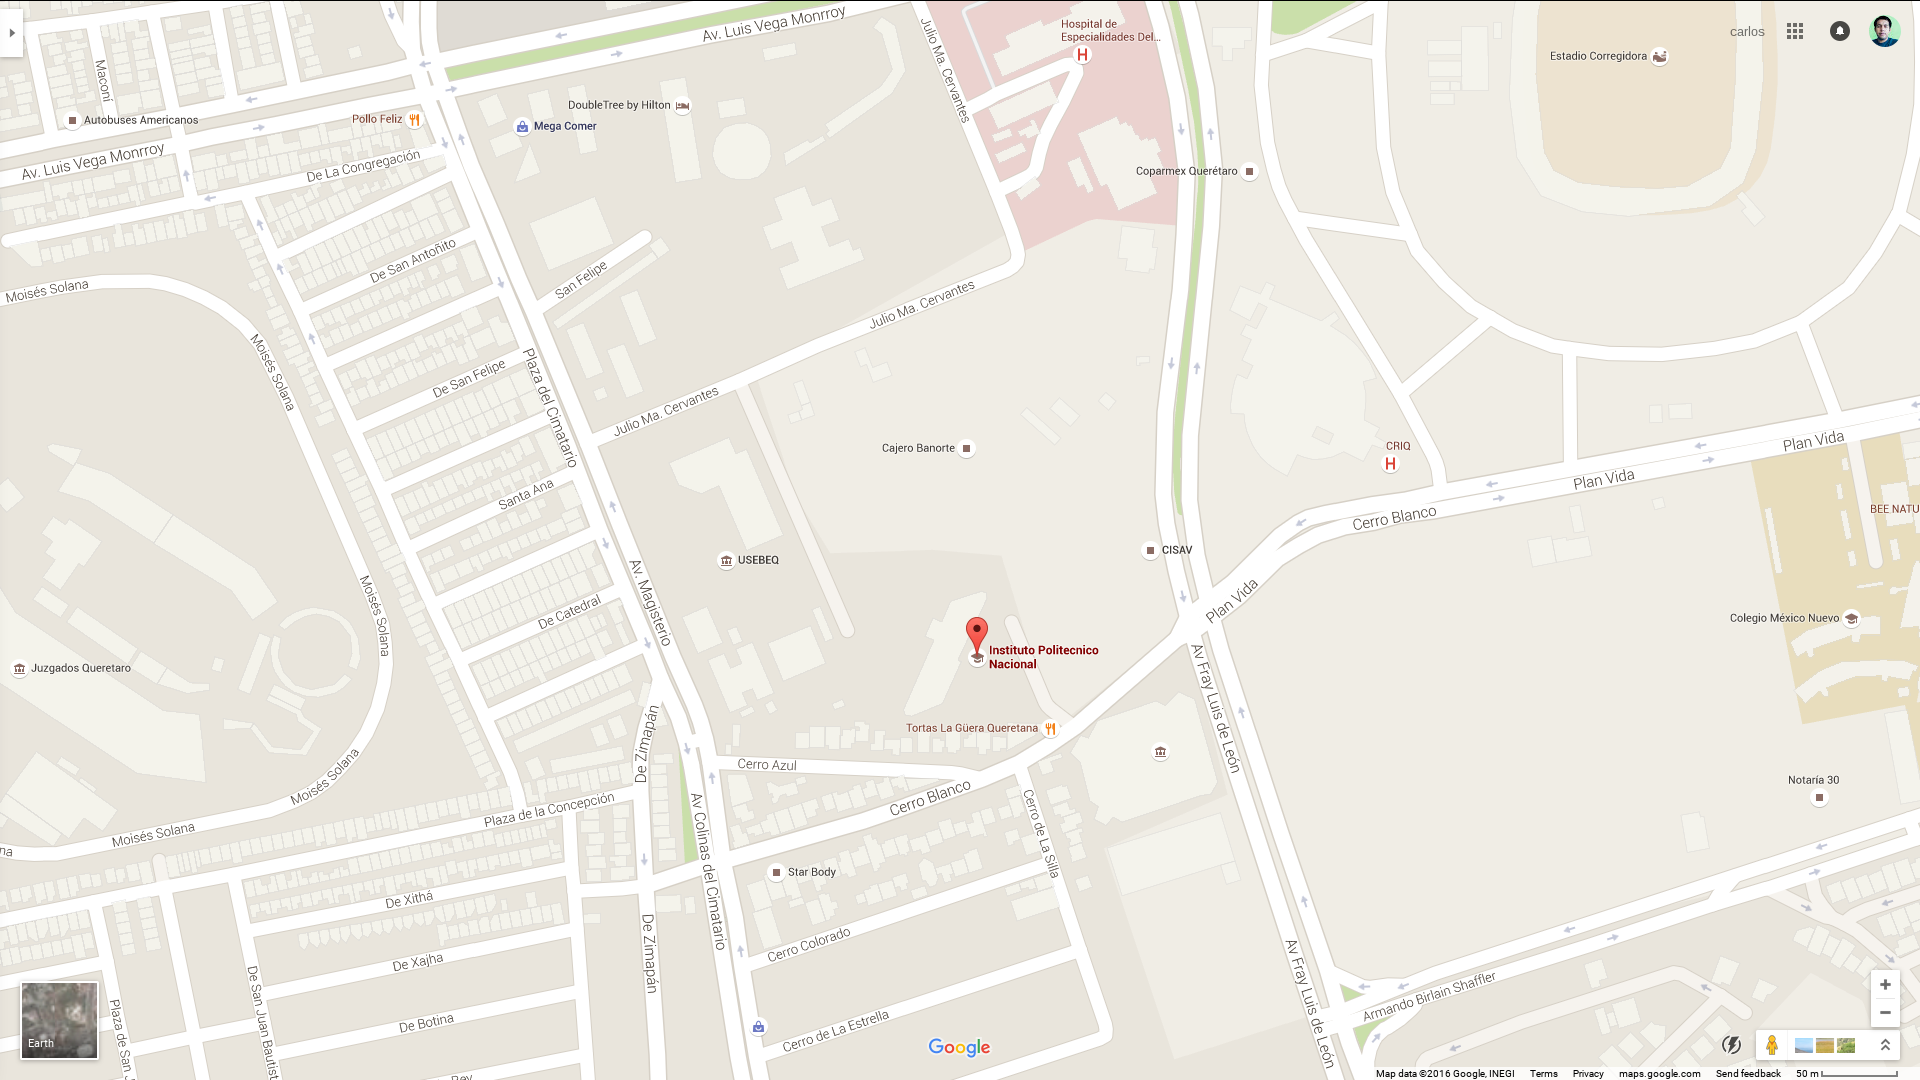
\includegraphics[width=0.9\textwidth]{./imagenes/cicata}
			 \end{center}
		\item[Teléfonos:] 1 (442) 2290804 o 01 (55) 5729 6000 Ext. 81002
		\item[E-Mail:] cicata@ipn.mx 
		\item[Fax:] 5395 4147
	\end{description}
		\subsubsection{Misión}
			Somos un centro de investigación creado por el IPN para fortalecer su impacto a nivel nacional, que atiende
			necesidades de formación de recursos humanos y de desarrollo tecnológico de la región, a través de proyectos
			de investigación que contribuyen al desarrollo social y a la competitividad de los sectores productivo y de
			servicios, con el respaldo de las capacidades del Instituto, con un enfoque multidisciplinario, innovador y
			de excelencia, en un marco de sustentabilidad.
		
		\subsubsection{Visión}
			En el 2025, el CICATA-Querétaro se ve como un centro de vanguardia en la investigación y formación de 
			recursos humanos; referente a nivel latinoamericano; con reconocimiento internacional por sus contribuciones
			de alto impacto y como una de las primeras opciones para alumnos e investigadores, por ser un centro
			innovador, competitivo, líder y emprendedor.
		
		\subsubsection{Valores}
			Hemos identificado un conjunto de valores que nos representan y que permiten cumplir nuestra misión y lograr
			la visión forjada:
			\begin{multicols}{2}
				\begin{itemize}
					\item Calidad
					\item Integridad
					\item Compromiso
					\item Asertividad
					\item Trabajo en equipo
					\item Aprendizaje continuo
				\end{itemize}
			\end{multicols}		
			
		\subsubsection{Objetivo}
			Servir de enlace entre la comunidad científica y los sectores productivos de bienes y servicios, atenderlos
			y ofrecerles soluciones a sus problemas de desarrollo. Para el cumplimiento de este objetivo, CICATA
			Querétaro desarrolla programas de investigación científica, tecnológica e innovación con un enfoque
			interdisciplinario, y asimismo atiende la formación de capital humano de alto nivel, contribuyendo
 			decisivamente al fortalecimiento de la calidad y la competitividad del aparato productivo mexicano.
 		
 		\subsubsection{Estructura Organizativa}
 			\begin{center}
			 	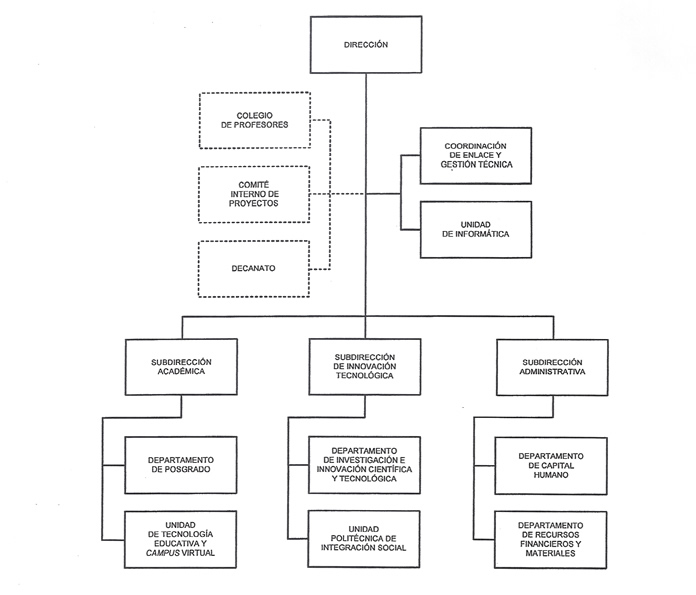
\includegraphics[width=0.9\textwidth]{./imagenes/organigrama}
			 \end{center}
			 
	
	\subsection{Descripción del departamento o área de trabajo}
		 El área de análisis de imágenes puede ser definida como la construcción de algoritmos para la extracción de 
		 información presente en las imágenes. Es un área donde una gran variedad de conceptos fundamentales necesitan 
		 ser desarrollado e importantes aplicaciones pueden crearse. Esta combinación de teoría y práctica es particularmente 
		 atractiva para CICATA Querétaro en virtud de corresponder con su objetivo operativo. El grupo de análisis de imágenes 
		 ha presentado desde sus orígenes resultados muy buenos en el renglón de vinculación y desarrollo tecnológico.  
		 Se han trabajado proyectos de vinculación con empresas e instituciones tales como TAMSA y el IFE, por mencionar algunos. 
		 En la actualidad con un grupo de cuatro investigadores esta tendencia se ha mantenido.  En este momento se estudian 
		 temas de interferometría, colorimetría, industrial, metrología, óptica, análisis de imágenes, procesamiento de imágenes, 
		 reconstrucción tridimensional e interpretación visual de la actividad.

\newpage
\section{Problemas a resolver}
	\begin{itemize}
		\item Amplificar áreas de la pantalla donde se enfoque la vista usando la vista.
		\item Detectar y seguir la dirección de la mirada.
		\item 
	\end{itemize}
\newpage
\section{Alcances y limitaciones}
	\subsection{Alcances}
		El sistema de seguimiento e identificación de la dirección de la mirada persigue el objetivo de permitir la interacción 
		usuario-maquina usando en el proceso únicamente los ojos y, proporcionar interactividad a esta parte del cuerpo.\\
		
		El uso directo e inmediato de la detección de la dirección de la mirada es el de proporcionar una forma interactiva 
		para magnificar zonas de la pantalla donde se enfoque la mirada en determinado momento.\\
		
		Inicialmente el sistema será desarrollado para funcionar en maquinas con sistema operativo Windows.\\
		
	\subsection{Limitaciones}
		Ciertamente el proyecto presenta algunas dificultades técnicas y algunas otras funcionales, entre las cuales encontramos
		las siguiente:\\
		
		Las condiciones no controladas, se espera unas condiciones de operación dentro de ciertos parámetros, es por tanto 
		importante considerar el rendimiento en entornos donde las mismas se encuentres fuera de norma, provocando un 
		funcionamiento incierto.\\
		
		La API de magnificación de Windows esta solo disponible en para arquitecturas de 32 bits, lo que imposibilita el desarrollo
		del sistema para arquitecturas de 64 bits.
		
		 

\chapter{FUNDAMENTACIÓN TEÓRICA}
\markboth{FUNDAMENTACIÓN TEÓRICA}{FUNDAMENTACIÓN TEÓRICA} 
\thispagestyle{empty}
\newpage
\section{Ingeniería del software}
	\subsection{Concepto de Software}
		Existen varias definiciones similares aceptadas para software, pero probablemente la más formal sea la siguiente:\\
		
		“Es el conjunto de los programas de cómputo, procedimientos, reglas, documentación y datos asociados que forman parte de las
		operaciones de un sistema de computación” (IEEE Std, 1993).\\
		
		Considerando esta definición, el concepto de software va más allá de los programas de computación en sus distintos estados: 
		código fuente, binario o ejecutable; también su documentación, los datos a procesar e incluso la información de usuario forman
		parte del software: es decir, abarca todo lo intangible, todo lo «no físico» relacionado.\\
		
		El término software fue usado por primera vez en este sentido por John W. Tukey en 1957. En la ingeniería de software y las
		ciencias de la computación, el software es toda la información procesada por los sistemas informáticos: programas y datos.
		
	\subsection{Clasificación del software \label{clasSoft}}
		Si bien la definición anterior de software es, en cierto modo arbitraria, y a veces confusa, a los fines prácticos se puede
		clasificar al software en tres grandes tipos \cite{IngSoft}:
		
	
		\begin{itemize}
			\item \textbf{Software de sistemas:} Su objetivo es desvincular adecuadamente al usuario y al programador de los detalles
			informáticos en particular que se use, aislándolo especialmente del procesamiento referido a las características internas de:
			memoria, discos, puertos y dispositivos de comunicaciones, impresoras, pantallas y teclados. El software de sistema le procura
			al usuario y programador adecuadas interfaces de alto nivel, controlador, herramientas y utilidades que permiten el 
			mantenimiento del sistema global. 
			
			Incluye entre otros:
			\begin{multicols}{2}
				\begin{itemize}
					\item Sistemas Operativos
					\item Controladores de dispositivos
					\item Herramientas de diagnostico
					\item Servidor de utilidades
					\item Herramientas de corrección y optimización.
				\end{itemize}
			\end{multicols}
			
			\item \textbf{Software de programación:} Es el conjunto de herramientas que permiten al programador desarrollar programas
			informáticos, usando diferentes alternativas y lenguajes de programación, de una manera práctica. Incluyen básicamente:
			\begin{multicols}{2}
				\begin{itemize}
					\item Editores de texto
					\item Compiladores
					\item Interpretes
					\item Enlazadores
					\item Depuradores
				\end{itemize}
			\end{multicols}
			\begin{itemize}
				\item Entornos de desarrollo integrado (\textsc{IDE}). Agrupan las anteriores herramientas, usualmente en un entorno
				visual, de forma que el programador no necesite introducir múltiples instrucciones para compilar , interpretar y depurar.
				Cuentan con una interfaz gráfica de usuario \textsc{GUI}.
			\end{itemize}
			
			\item \textbf{Software de aplicacion:} es aquel que permite a los usuarios llevar a cabo una o varias tareas específicas, en
			cualquier campo de actividad susceptible de ser automatizadas o asistido, con especial énfasis en los negocios. Incluye entre
			muchos otros:
			\begin{multicols}{2}
				\begin{itemize}
					\item Control de sistemas.
					\item Automatización industrial
					\item Software educativo
					\item Software empresarial
					\item Base de datos
					\item Telecomunicaciones
					\item Videojuegos
					\item Software medico
					\item Aplicaciones ofimáticas
					\item Software de calculo numérico y simbólico
					\item Diseño asistido (\textsc{CAD})
				\end{itemize}
			\end{multicols}
		\end{itemize}
		
	\subsection{Concepto de la Ingeniería de Software}
		La ingeniería de software es una disciplina de la ingeniería que comprende todos los aspectos de la producción de software desde 
		las etapas iniciales de la especificación del sistema, hasta el mantenimiento de éste después de que se utiliza.
		En esta definición existen dos frases clave:
		\begin{description}
			\item[Disciplina de la ingeniería: ] Los ingenieros hacen que las cosas funcionen. Aplican teorías, métodos y herramientas 	
			donde sean convenientes, pero las utiliza de forma selectiva y siempre tratando de descubrir soluciones a los problemas, aun 
			cuando no existan teorías o métodos aplicables para resolverlos.
			\item[Todos los aspectos de producción de software: ] La ingeniería de software no solo comprende los procesos técnicos del 
			desarrollo de software, sino también actividades tales como la gestión de proyectos de software y el desarrollo de 
			herramientas, métodos y teorías de apoyo a la producción de software.
		\end{description}		 
		en general los ingenieros de software adoptan un enfoque sistemático y organizado en su trabajo, ya que es la forma mas efectiva
		de producir software de calidad \cite{IngSoft} pp.6.
\newpage
\section{Herramientas de desarrollo}
	Como se describe en la sección \ref{clasSoft} hay diferentes clases y tipos de software, entre los que se encuentran las herramientas
	de 	desarrollo o software de desarrollo, así como software de aplicación, en este proyecto se han usado variedad de ellas, de las 
	cuales se da una descripción a continuación:
	\subsection*{Software de desarrollo}	
	\subsection{Visual Studio Community 2015 \label{VS}}
		\textsc{Visual Studio Community 2015} es un entorno de desarrollo integrado creado y distribuido por \textsc{Microsoft}, 
		para el sistema operativo de la misma.
		Soporta una gran variedad de lenguajes de programación tales como, \textsc{ C++, C\#, Visual Basic, .NET, F\#, Java, Python, 
		Ruby, PHP}, al igual que entornos de desarrollo web como \textsc{ASP.NET MVC, Django, etc.,} a lo cual sumarle las nuevas
		capacidades online bajo Windows Azure en forma del editor Monaco.
		Esta version en particular tiene la particularidad de ser gratuita e incluir todas las características de la versión 
		\textsc{Express}, enfocada en desarrolladores individuales, proyectos de código abierto, investigación académica, educación
		y pequeños equipos  de profesionales.
		
	\subsection{Qt Creator \label{qt}}
	Qt Creator es un IDE (entorno de desarrollo integrado) multiplataforma que se ajusta a las necesidades de los desarrolladores Qt. 
	Este es parte de Qt Project \footnote{\textit{\scriptsize \href{http://www.qt.io/}{Qt Project}}}.
	
	Qt Creator se centra en proporcionar características que ayudan a los nuevos usuarios de Qt a aprender y comenzar a desarrollar
	rápidamente, también aumenta la productividad de los desarrolladores con experiencia en Qt.
	\begin{multicols}{2}
	\begin{itemize}
		\item Editor de código con soporte para C+, QML y ECMAscript
		\item Herramientas para la rapida navegacion del codigo
    	\item Resaltado de sintaxis y auto-completado de código
		\item Control estático de código y estilo a medida que se escribe
	    \item Soporte para refactoring de código
    	\item Ayuda sensitiva al contexto
	    \item Plegado de código (code folding)
    	\item Paréntesis coincidentes y modos de selección
	\end{itemize}
	\end{multicols}
	
	\subsection{PyCharm \label{pych}}
		\textsc{Pycharm} es un entorno integrado de desarrollo (\textsc{IDE}) usado para la programacion en \textsc{Python} (\ref{python}). 
		Provee herramientas de análisis de código, depurador gráfico, pruebas unitarias, integración con sistemas de control de versiones
		y soporte para el desarrollo con \textsc{Django}.\\
		Desarrollado por la compañía \href{https://en.wikipedia.org/wiki/JetBrains}{JetBrains}
		\footnote{\scriptsize JetBrains: https://en.wikipedia.org/wiki/JetBrains}.\\
		
		Es multi-plataforma, funcionando en Windows, Mac OS X y Linux, cuenta con una version profesional liberada bajo licencia 
		propietaria y con una versión comunitaria bajo los términos de \href {https://en.wikipedia.org/wiki/Apache_License}{Apache Licence}
		\footnote{\scriptsize Apache: https://en.wikipedia.org/wiki/Apache\_License}, aunque esta última cuenta con algunas limitaciones.\\
		
		Entre sus características mas destables se encuentran las siguientes:
		\begin{multicols}{2}
		\begin{itemize}
			\item Asistencia en el análisis de código
			\item Auto-completado de código
			\item Errores de sintaxis
			\item Resaltado de lineas
			\item Vistas de navegación
			\item Vistas de estructuras
			\item Integración con Python Debugguer.
			\item Integración con CVS.
		\end{itemize}
		\end{multicols}
		
	\subsection{Sublime-Text \label{subl}}
		Sublime Text es un editor de texto y editor de código fuente está escrito en C++ y Python para los plugins. Desarrollado
		originalmente como una extensión de \texttt{Vim}, con el tiempo fue creando una identidad propia, por esto aún conserva un modo 
		de edición tipo vi llamado Vintage mode.\\
		
		Características:
		\begin{multicols}{2}
			\begin{itemize}
				 \item Minimapa. consiste en una previsualización de la estructura del código
				 \item Multi selección: Hace una selección múltiple de un término por diferentes partes del archivo.
				 \item Multi cursor: Crea cursores con los que podemos escribir texto de forma arbitraria en diferentes posiciones del
				 	   archivo.
				 \item Multi layout: Trae siete configuraciones de plantilla podemos elegir editar en una sola ventana o hacer una división
				 \item Soporte nativo para infinidad de lenguajes: Soporta de forma nativa 43 lenguajes de programación y texto plano.
				 \item Remarcado de sintaxis: El remarcado de sintaxis es completamente configurable a través de archivos de configuración 
				 	   del usuario.
				 \item Búsqueda dinámica: Se puede hacer búsqueda de expresiones regulares o por archivos, proyectos, directorios, una 
				 	   conjunción de ellos o todo a la vez.
				 \item Keybindings: Todas las teclas pueden ser sobrescritas a nuestro gusto.
				 \item Etc.
			\end{itemize}
		\end{multicols}
		
		Se puede descargar desde el sitio web \href{https://www.sublimetext.com/}{Sublime-Text} 
		\footnote{\scriptsize Subl-Text: https://www.sublimetext.com/}
		y evaluar de forma gratuita. Sin embargo no es software libre o de código abiertoy se debe obtener una licencia 	para su uso
		continuado, aunque la versión de evaluación es plenamente funcional y no tiene fecha de caducidad.
				
		
		
	\subsection{Rstudio \label{RS}}
		RStudio es un entorno de desarrollo integrado (\textsc{IDE}) para R (\ref{r}).\
		Esta disponible de forma libres y en edición comercial, se ejecuta en entornos multiplataforma (Windows, Mac OS X y Linux) o
		sobre navegadores web conectados a \textsc{RStudio Server o RStudio Server Pro (Debian/Ubuntu, RedHat/CentOS y SUSE Linux)}.\\
		
		RStudio tiene la misión de proporcionar el entorno informático estadístico R. Permite un análisis y desarrollo para que 
		cualquiera pueda analizar los datos con R.
		
		Entre sus características se encuentran la siguientes:
		\begin{multicols}{2}
			\begin{itemize}
				\item Consola integrada
				\item Resaltado de sintaxis
				\item Ejecución directa de código R.
				\item Herramientas para gráficos
				\item Historial
				\item Depurador interactivo
				\item Fácil administración de espacios de trabajo.
				\item Ayuda y documentación integrada
				\item Edición con Sweave y R Markdown
			\end{itemize}
		\end{multicols} 
		Esta disponible desde la web oficial del proyecto \href{https://www.rstudio.com/}{RStudio} 
		\footnote{\scriptsize RStudio: https://www.rstudio.com/} en sus dos versiones.\\
		
		
	
	\subsection{CMake \label{CM}}
		CMake es una herramienta multiplataforma de generación o automatización de código. El nombre es una abreviatura para 
		\textit{'cross platform make' (make multiplataforma)}; más allá del uso de \textit{'make'} en el nombre, CMake es una suite separada 
		y de más alto nivel que el sistema \texttt{make} común de Unix, siendo similar a las autotools.
		
		CMake es una familia de herramientas diseñada para construir, probar y empaquetar software. CMake se utiliza para controlar el
		proceso de compilación del software usando ficheros de configuración sencillos e independientes de la plataforma. 
		
		Desarrollado por \textit{Andy Cedilnik, Bill Hoffman, Brad King, Ken Martin, Alexander Neundorf} se puede acceder a la ultima 
		version estable en \href{www.cmake.org}{CMake} \footnote{\scriptsize CMake: www.cmake.org}.\\
		
		Entre las principales funcionalidad se encuentran las siguientes:
		\begin{multicols}{2}
			\begin{itemize}
				\item Ficheros de configuración escritos en un lenguaje de scripting específico para CMake
				\item Análisis automático de dependencias para C, C++, Fortran, y Java
				\item Soporte para SWIG, Qt, FLTK, a través del lenguaje de scripting de CMake
				\item Soporte para varias versiones de Microsoft Visual Studio, incluyendo la 6, 7, 7.1, 8.0, 9.0 y 10.0
				\item Detección de cambios en ficheros usando timestamps tradicionales
				\item Soporte para builds paralelos
				\item Compilador cruzado
				\item Soporte para builds multiplataforma
				\item Integrado con \textsc{DART (software), CDash, CTest y CPack}, una colección de herramientas para prueba y liberación
				 de software
			\end{itemize}
		\end{multicols}
		
	\subsection*{Software de aplicación}
	
	\subsection{Sistema de control de versiones Git \label{git}}
		Git es un software de control de versiones diseñado por \textit{Linus Torvalds}, pensando en la eficiencia y la confiabilidad del
		mantenimiento de versiones de aplicaciones cuando éstas tienen un gran número de archivos de código fuente. Al principio, Git se
		pensó como un motor de bajo nivel sobre el cual otros pudieran escribir la interfaz de usuario o front end como Cogito o StGIT. 
		
		Sin embargo, Git se ha convertido desde entonces en un sistema de control de versiones con funcionalidad plena. Hay algunos
		proyectos de mucha relevancia que usan Git, en particular, el grupo de programación del núcleo Linux.
		
		Entre las características más relevantes se encuentran:
		\begin{multicols}{2}
			\begin{itemize}
				\item Fuerte apoyo al desarrollo no lineal, por ende rapidez en la gestión de ramas y mezclado de diferentes versiones. 
				\item Gestión distribuida, Git le da a cada programador una copia local del historial del desarrollo entero, y los 
				cambios se propagan entre los repositorios locales. 
				\item Los almacenes de información pueden publicarse por HTTP, FTP, rsync o mediante un protocolo nativo, ya sea a través 
				de una conexión TCP/IP simple o a través de cifrado SSH.
				\item Gestión eficiente de proyectos grandes, dada la rapidez de gestión de diferencias entre archivos.
			\end{itemize}
		\end{multicols}
		
		La documentación completa, tutoriales de uso y medios de instalación se pueden encontrar en la pagina oficial de 
		\href{https://git-scm.com/}{Git} \footnote{\scriptsize Git: https://git-scm.com/}
	
		
	\subsection{MariaDB \label{maria}}
		\textsc{MariaDB} es un sistema de gestión de bases de datos derivado de \textsc{MySQL} con licencia \textsc{GPL}. 
		Está desarrollado por \textit{Michael (Monty) Widenius (fundador de MySQL)} y la comunidad de desarrolladores de software 
		libre. 
		
		Introduce dos motores de almacenamiento nuevos, uno llamado Aria -que reemplaza con ventajas a \textsc{MyISAM}- y otro
		lamado \textsc{XtraDB} -en sustitución de \textsc{InnoDB}. Tiene una alta compatibilidad con MySQL ya que posee las mismas
		órdenes, interfaces, APIs y bibliotecas, siendo su objetivo poder cambiar un servidor por otro directamente. 
		Este \textsc{SGBD} surge a raíz de la compra de \textit{Sun Microsystems}.
		
		MariaDB es un fork directo de MySQL que asegura, permanecerá una versión de este producto con licencia GPL. 
		La ultima versión estable se puede encontrar en la web oficial del proyecto \href{https://mariadb.org/}{MariaDB} 
		\footnote{\scriptsize MariaDB: https://mariadb.org/}.
		
	\subsection{SQLite}
		\textsc{SQLite} es un sistema de gestión de bases de datos relacional compatible con \textsc{ACID}, contenida en una
		relativamente pequeña (~275 kiB) biblioteca escrita en C. SQLite es un proyecto de dominio público creado por 
		\textit{D. Richard Hipp}.
		
		A diferencia de los sistema de gestión de bases de datos cliente-servidor, el motor de SQLite no es un proceso independiente 
		con el que el programa principal se comunica. En lugar de eso, la biblioteca SQLite se enlaza con el programa pasando a ser
		parte integral del mismo. 
		
		El programa utiliza la funcionalidad de SQLite a través de llamadas simples a subrutinas y funciones. Esto reduce la latencia 
		en el acceso a la base de datos, debido a que las llamadas a funciones son más eficientes que la comunicación entre procesos. 
		El conjunto de la base de datos (definiciones, tablas, índices, y los propios datos), son guardados como un sólo fichero
		estándar en la máquina cliente. 
		Este diseño simple se logra bloqueando todo el fichero de base de datos al principio de cada transacción.
		
		En su versión 3, SQLite permite bases de datos de hasta \textsc{2 Terabytes} de tamaño, y también permite la inclusión de campos
		tipo \textsc{BLOB}.
		
	\subsection*{Librerías}	
	
	\subsection{OpenCV \label{cv}}
			
		
		\textsc{OpenCV} es una biblioteca libre de visión artificial originalmente desarrollada por \textsc{Intel}. 
		Desde que apareció su primera versión alfa en el mes de enero de 1999, se ha utilizado en infinidad de aplicaciones. 
		Desde sistemas de seguridad con detección de movimiento, hasta aplicaciones de control de procesos donde se requiere
		reconocimiento de objetos. Esto se debe a que su publicación se da bajo licencia \textsc{BSD}, que permite que sea usada
		libremente para propósitos comerciales y de investigación con las condiciones en ella expresadas.
		
		OpenCV es multiplataforma, existiendo versiones para \textsc{GNU/Linux, Mac OS X y Windows}. Contiene más de 500 funciones 
		que abarcan una gran gama de áreas en el proceso de visión, como reconocimiento de objetos (reconocimiento facial), 
		calibración de cámaras, visión estérea y visión robótica.
		
		El proyecto pretende proporcionar un entorno de desarrollo fácil de utilizar y altamente eficiente. Esto se ha logrado
		realizando su programación en código C y C++ optimizados, aprovechando además las capacidades que proveen los procesadores
		multinúcleo. OpenCV puede además utilizar el sistema de primitivas de rendimiento integradas de Intel, un conjunto de 
		rutinas de bajo nivel específicas para procesadores Intel \textsc{(IPP)}.
		
		
	\subsection{IntraFace}
		IntraFace es una librería que incluye algoritmos para análisis de patrones faciales, se comenzó a desarrollar en 2010 en la
		universidad \textsc{Carnigie Mellon \& University of Pittsburgh}, actualmente la ultima version de la misma es la 1.0, soportada 
		por Human Sensing Laboratory.\\
		Para este proyecto se usa una version anterior de la misma, provista para fines educativos y/o investigación sin fines de lucro.

	
		
\newpage		
	
\section{Lenguajes de programación}
	
	Un lenguaje de programación es una herramienta que nos permite comunicarnos e instruir a la computadora para que realice una tarea
	especifica. Cada lenguaje de programación posee una sintaxis y un léxico particular, es decir, la forma de escribirse, que es 
	diferente en cada uno por la forma en que fue creado y por la forma que trabaja su compilador para revisar, acomodar y reservar el
	programa en memoria.
	
	Existen muchos lenguajes, sin embargo en este proyecto solo nos interesan los siguientes:
	\begin{multicols}{3}	
		\begin{itemize}
			\item C++
			\item Python
			\item R		
		\end{itemize}
	\end{multicols}
	
	\subsection{C++}
		\textsc{C++} es un lenguaje de programación diseñado a mediados de los años 1980 por \textit{Bjarne Stroustrup}. La intención 
		de su creación fue el extender al lenguaje de programación \textsc{C}, agregando mecanismos que permitieran la manipulación de
		objetos. En ese sentido, desde el punto de vista de los lenguajes orientados a objetos, el C++ es un lenguaje híbrido, por un lado 
		es un lenguaje que sigue muy ligado a hardware subyacente, manteniendo una considerable potencia para la programación a bajo nivel, 
		pero se le han añadido elementos que le permiten un estilo de programación de alto nivel de abstracción.
		
		La definición oficial nos dice que C++ es un lenguaje de propósito general basado en C, al que se le han añadido nuevos tipos de 
		datos, plantillas, clases, mecanismos de acepciones, espacio de nombres (STD), funciones inline, sobrecarga de operadores, 
		referencias, manejo de memoria persistente y algunas utilidades adicionales en la librería estándar de C++.
		
		\subsubsection{Historia}
			El comité para el estándar ANSI C fue formado en 1983 con el objetivo de crear un lenguaje uniforme a partir del C original,
			desarrollado por \textit{Kernighan y Ritchie} en 1972, en la AT\&T. Hasta entonces el estándar lo marcaba el libro escrito en
			1978 por estos dos autores. 
			El lenguaje C++ se comenzó a desarrollar en 1980. Su autor fue Bjarne Stroustrup, también de la AT\&T. 
			Al comienzo era una extensión del lenguaje C que fue denominada \textit{C with classes}. Este nuevo lenguaje comenzó a ser
			utilizado fuera de la AT\&T en 1983. El nombre C++ es también de ese año, y hace referencia al carácter del operador incremento
			de C (++). Ante la gran difusión y éxito que iba obteniendo en el mundo de los programadores, la AT\&T comenzó a estandarizarlo
			internamente en 1987. En 1989 se formó un comité ANSI (seguido algún tiempo después por un comité ISO) para estandarizarlo a
			nivel americano e internacional.
			
		 \subsubsection{Características}
		 	Antes, mencionar que tanto C como C++ son lenguajes compilados, y no interpretados. Esta diferencia es muy importante, ya que
		 	afecta mucho a muchos aspectos relacionados con la ejecución del programa.\\
		 	
		 	Como lenguaje de programación orientado a objetos  se basa en una filosofía completamente diferente a la se su predecesor, exige 
		 	el cambio completo de paradigma al programador, las propias características de la Programación Orientada a Objetos de C++ son 
		 	la causa principal de ello.
		 \subsubsection{Conceptos generales de POO}
		 	La programación orientada a objetos (POO) se fundamenta en algunos principios o pilares que la definen:
		 	\begin{description}
		 		\item[Clase:] Es una plantilla que define la estructura de un conjunto de objetos, que al ser creados se llamarán las
			 		instancias de la clase. Esta estructura está compuesta por la definición de los atributos y la implementación de las
			 		operaciones (métodos).
		 		\item[Objeto:] Es la implementación de una instancia de clase, es decir, una ocurrencia de esta, que tiene los atributos
		 			definidos por la clase, y sobre la que se puede ejecutar las operaciones definidas en ella. 
		 		\item[Identidad:] Característica de cada objeto que lo diferencia de los demás, incluyendo de aquellos que pudieran
		 			s pertenecer a la misma clase y tener los mismos valores en sus atributos. 
		 		\item[Herencia:] Es la capacidad que tienen las clases para heredar propiedades y métodos de otras clases. 
		 	\end{description}
		
		
	\subsection{Python \label{python}}
		Python es un lenguaje de programación creado por Guido van Rossum a principios de los años 90 cuyo nombre está inspirado en el grupo
		de cómicos ingleses \textit{Monty Python}. Es un lenguaje similar a Perl, pero con una sintaxis muy limpia y que favorece un código 
		legible \cite{python}.
		
		Se trata de un lenguaje interpretado o de script, con tipado dinámico, fuertemente tipado, multiplataforma y orientado a objetos.\\
		
		El intérprete de Python está disponible en multitud de plataformas (\textsc{UNIX, Solaris, Linux, DOS, Windows, OS/2, Mac OS}, etc.)
		por lo que si no utilizamos librerías específicas de cada plataforma nuestro programa podrá correr en todos estos sistemas sin
		grandes cambios.\\
		Python es un lenguaje que todo el mundo debería conocer. Su sintaxis simple, clara y sencilla; el tipado dinámico, el gestor de
		memoria, la gran cantidad de librerías disponibles y la potencia del lenguaje, entre otros, hacen que desarrollar una aplicación en
		Python sea sencillo, muy rápido y, lo que es más importante, divertido.\\		
		
		Python no es adecuado sin embargo para la programación de bajo nivel o para aplicaciones en las que el rendimiento sea crítico.\\
		Algunos casos de éxito en el uso de Python son Google, Yahoo, la NASA, Industrias Ligh \& Magic, y todas las distribuciones Linux, 
		en  las que Python cada vez representa un tanto por ciento mayor de los programas disponibles.
		
		\subsubsection{Instalacion de Python}
			Existen varias implementaciones distintas de Python: CPython, Jython, IronPython, PyPy, etc	
			
			CPython es la más utilizada, la más rápida y la más madura. Cuando la gente habla de Python normalmente se refiere a esta
			implementación. 
			En este caso tanto el intérprete como los módulos están escritos en C.\\
			
			Jython es la implementación en Java de Python, mientras que IronPython es su contrapartida en C\# (.NET). Su interés estriva en 
			que utilizando estas implementaciones se pueden utilizar todas las librerías disponibles para los programadores de Java y .NET.

			PyPy, por último, como habréis adivinado por el nombre, se trata de una implementación en Python de Python.
			
			CPython está instalado por defecto en la mayor parte de las distribuciones Linux y en las últimas versiones de Mac OS. Para
			comprobar si está instalado abre una terminal y escribe \texttt{python}. Si está instalado se iniciará la consola interactiva 
			de Python y obtendremos parecido a lo siguiente:
			
			\begin{minipage}[t]{0.3\textwidth}
			\scriptsize			
				\begin{verbatim}

					Python 3.5.1 (default, Mar  3 2016, 09:29:07)
					[GCC 5.3.0] on linux
					Type "help", "copyright", "credits" or "license" for more information.
					>>> |
				\end{verbatim}			
			\end{minipage}
			\\
			si no te muestra algo parecido no te preocupes, instalar Python es muy sencillo. Puedes descargar la versión correspondiente a
			tu sistema operativo desde la web de \href{https://www.python.org/}{Python} 
			\footnote{\scriptsize Python: https://www.python.org/}.
			
			\subsubsection{Herramientas básicas}
				Existen dos formas de ejecutar código Python. Podemos escribir líneas de código en el intérprete y obtener una respuesta del
				intérprete para cada línea (sesión interactiva) o bien podemos escribir el código de un programa en un archivo de texto y
				ejecutarlo.
				
				Para el trabajo del proyecto se uso PyCharm (\ref{pych}) como IDE de desarrollo, anque en algunas ocaciones se uso editor de
				texto, \textsc{Sublime-text} (\ref{subl}) , para la edición rápida.

	\subsection{R \label{r}}
		R es una implementación de software libre del lenguaje S pero con soporte de alcance estático. Se trata de uno de los
		lenguajes más utilizados en investigación por la comunidad estadística, siendo además muy popular en el campo de la minería de
		datos, la investigación biomédica, la bioinformática y las matemáticas financieras. A esto contribuye la posibilidad de cargar
		diferentes bibliotecas o paquetes con funcionalidades de cálculo o graficación \cite{rdev} .
		
		R es parte del sistema GNU y se distribuye bajo la licencia GNU GPL. Está disponible para los sistemas operativos Windows,
		Macintosh, Unix y GNU/Linux.
		
		
	
		
\newpage
\section{Metodologías de desarrollo de software}
	
	\subsection{Metodología de desarrollo extremo \label{XP}}
		La programación extrema se basa en una serie de reglas y principios que se han ido gestando a lo largo de toda la historia de la 
		ingeniería del software. Usadas conjuntamente proporcionan una nueva metodología de desarrollo software que se puede englobar dentro
		de las metodologías ligeras, que son aquéllas en la que se da 	prioridad a las tareas que dan resultados directos y que reducen la
		burocracia que hay alrededor tanto como sea posible (pero no más).
		La programación extrema, dentro de las metodologías ágiles, se puede clasificar dentro de las evolutivas.
		
		Una de las características de \textsc{eXtreme Programming} es que muchos de, si no todos, sus ingredientes son de sobra conocidos
		dentro de la rama de la ingeniería del software desde hace tiempo, incluso desde sus comienzos. Los autores de han seleccionado los
		que han considerados como los mejores y han profundizado en sus relaciones y en cómo se refuerzan unos a otros. El resultado ha sido
		una metodología única y compacta. Por eso, aunque se pueda alegar que la programación extrema no se base en	principios nada nuevos,
		se ha de aclarar que, en conjunto, es una nueva forma de ver el desarrollo de software. 
		
		\subsubsection{El proceso de desarrollo extremo}
			La programación extrema parte del caso habitual de una compañía que desarrolla software, generalmente software a medida, en la
			que hay diferentes roles: un equipo de gestión, un equipo de desarrolladores y los clientes. La relación con el cliente es
			totalmente diferente a lo que se ha venido haciendo en las metodologías tradicionales que se basan fundamentalmente en una fase
			de captura de requisitos previa al desarrollo y una fase de validación posterior al mismo. 
			
		\subsubsection{Interacción con el cliente }
			En la programación extrema al cliente no sólo se le pide que apoye al equipo de desarrollo, en realidad podríamos decir que es
			parte de él. Su importancia es capital a la hora de abordar las historias de los usuarios y las reuniones de planificación, como
			veremos más adelante. Además, será tarea suya retroalimentar al equipo de desarrolladores después de cada iteración con los
			problemas con los que se ha encontrado, mostrando sus prioridades, expresando sus sensaciones... Existirán métodos como pruebas
			de aceptación que ayudarán a que la labor del cliente sea lo más fructífera posible.
			
			
			En resumen, el cliente se encuentra mucho más cercano al proceso de desarrollo. Se elimina la fase inicial de captura de
			requisitos y se permite que éstos se vayan definiendo de una forma ordenada durante el tiempo que dura el proyecto. 
			El cliente puede cambiar de opinión sobre la marcha y a cambio debe encontrarse siempre disponible para resolver dudas del
			equipo de desarrollo y para detallar los requisitos especificados cuando sea necesario. 
			
			El proceso de captura de requisitos de XP gira entorno a una lista de características que el cliente desea que existan en el
			sistema final. Cada una de estas características recibe el nombre de historias de usuarios y su definición consta de dos fases:
						
			\begin{description}
				\item[En la primera fase] el cliente describe con sus propias palabras las características y el responsable del equipo de
					desarrollo le informa de la dificultad técnica de cada una de ellas y por lo tanto de su coste.
				\item[La segunda fase] consiste en coger las primeras historias que serán implementadas (primera iteración) y dividirlas 
					en las tareas necesarias para llevarlas a 	cabo.
			\end{description}
			
			Este proceso es una de las principales diferencias con las metodologías tradicionales. Aunque las historias de usuarios guardan
			cierta relación con otras técnicas como los casos de uso de UML, su proceso de creación es muy diferente. En lo que al cliente
			se refiere no se le exige que especifique exactamente lo que quiere al principio con un documento de requisitos de usuario. La
			parte que se mantiene con este documento es que es el cliente el que tiene que escribir lo que quiere, no se permite que alguien
			del equipo de desarrolladores lo escriba por él.
			
		\subsubsection{Planificación del proyecto}
			La planificación debe de seguir unas ciertas premisas. La primordial es que las entregas se hagan cuanto antes y que con cada
			iteración el cliente reciba una nueva  versión. Cuanto más tiempo se tarde en introducir una parte esencial, menos tiempo habrá
			para trabajar en ella posteriormente. Se aconsejan muchas entregas y muy frecuentes. De esta forma, un error en una parte
			esencial del sistema se encontrará pronto y, por tanto, se podrá arreglar antes.\\
			
			Sin embargo, los requisitos anteriores en cuanto a la planificación no deben suponer horas extra para el equipo de desarrollo.\\
			
			Pero lo mejor de todo es que a la hora de planificar uno se puede equivocar. Es más, todos sabemos que lo común es equivocarse y
			por ello la metodología ya tiene previsto mecanismos de revisión. Por tanto, es normal que cada 3 a 5 iteraciones se tengan que
			revisar las historias de los usuarios y re-negociar nuevamente la planificación.\\
			
		\subsubsection{Diseño, desarrollo y pruebas}
			El desarrollo es la pieza clave de todo el proceso de programación extrema. Todas las tareas tienen como objetivo que se
			desarrollo a la máxima velocidad, sin 	interrupciones y siempre en la dirección correcta. 
			También se otorga una gran importancia al diseño y establece que éste debe ser revisado y mejorado de forma continua según se
			van añadiendo funcionalidades al sistema
			
			La clave del proceso de desarrollo de XP es la comunicación. La gran mayoría de los problemas en los proyectos de desarrollo son
			provocados por falta de comunicación en el equipo, así que se pone un gran énfasis en facilitar que la información fluya lo más
			eficientemente posible. 
			
			Como ya hemos visto con anterioridad, uno de los principios de la programación extrema es la simplicidad. El diseño debe ser lo
			más simple posible, pero no más simple. El paradigma KISS (\textit{'Keep It Small and Simple'})se lleva hasta las últimas 
			consecuencias. Por ejemplo, se hace énfasis en no añadir funcionalidad nunca antes de lo necesario, por las sencillas razones 
			de que probablemente ahora mismo no sea lo más prioritario o porque quizás nunca llegue a ser necesaria.
			
			
			Supongamos que ya hemos planificado y dividido en tareas, como se ha comentado en los párrafos anteriores. Lo lógico sería
			empezar ya a codificar. Pues no. Nos encontramos con otro de los puntos clave de la programación extrema (y que sí es innovador
			en ella): las pruebas unitarias se implementan a la vez hay que el código de producción. De hecho cada vez que se va a
			implementar una pequeña parte se escribe una prueba sencilla y luego el código suficiente para que la pase. Cuando la haya
			pasado se repite el proceso con la siguiente parte.
			
			Esta forma de usar las pruebas unitarias ayuda a priorizar y comprobar la evolución del desarrollo y que ofrecen 
			retroalimentación inmediata. Ya no hay imprescindibles dos equipos diferenciados que desarrollan y prueban cada uno por su
			cuenta. Ahora el ciclo se  basa en implementar una prueba unitaria, codificar la solución y pasar la prueba, con lo que se
			consigue un código simple y funcional de manera bastante rápida. Por eso es importante que las pruebas se pasen siempre al 100%.
			
			Las pruebas unitarias no se han de confundir con las pruebas de aceptación que han sido mencionadas con anterioridad. Éstas
			últimas son pruebas realizadas por el cliente o por el usuario final para constatar que el sistema hace realmente lo que él
			quiere.
			 
			La programación extrema viene a perseguir lo que se ha venido a llamar integración continua. De esta forma, haciéndolo cada vez
			con pequeños fragmentos de código, se evita la gran integración final. 
			
			En todo desarrollo de programación extrema debería existir, por tanto, una versión siempre integrada a la sincronización por
			parte de los desarrolladores con el repositorio central debe darse como mínimo una vez al día, de manera que los cambios siempre
			se realicen sobre la última versión. De esta forma nos podemos asegurar de que las modificaciones que hacemos no se estén
			haciendo sobre una  versión obsoleta\\
			
			El proceso de desarrollo no lo va a hacer un desarrollador en solitario, sino siempre con otra persona, algo que se ha venido a 
			llamar programación por parejas. Una pareja de desarrolladores debe compartir ordenador, teclado y ratón. El principal objetivo 
			es realizar de forma continua y sin parar el desarrollo una revisión de diseño y de código. Las parejas deben ir rotando de
			forma periódica para hacer que el conocimiento del sistema se vaya difundiendo por el equipo (facilitándose que el código sea 
			de todos), a la vez que se fomentan el entrenamiento cruzado.
			
		\subsubsection{Resumen de XP}
			Todos los punto anteriormente detallados, bien los podemos definir y resumir en la siguiente lista, obviamente cada uno de 
			ellos lleva consigo un gran significado de fondo, pero en general  y conociendo la metodología se puede uno basar en la
			siguiente lista para cerciorarse de que se están cumpliendo los puntos que la metodología estipula que se deben llevar a cabo.
			\begin{multicols}{2}
				\begin{enumerate}
					\item El juego de la planificación (the planning game).
					\item Pequeñas entregas (small releases).
					\item Metáfora (metaphor).
					\item Diseño simple (simple design).
					\item Pruebas (testing).
					\item Refactorización (refactoring).
					\item Programación por parejas (pair programming).
					\item Propiedad colectiva (collective ownership).
					\item Integración continua (continous integration).
					\item 40 horas semanales (40-hour week).
					\item Cliente en casa (on-site costumer).
					\item Estándares de codificación (coding standards).
				\end{enumerate}
			\end{multicols}
			
			Se puede considerar como el resumen de bolsillo de la metodología de desarrollo extremo, y llevarla a cada lugar en el que se este desarrollando.


\chapter{DESCRIPCIÓN DE ACTIVIDADES REALIZADAS}
\markboth{ACTIVIDADES REALIZADAS}{ACTIVIDADES REALIZADAS}
\thispagestyle{empty}
\newpage
\section{Análisis}

\section{Diseño}

\section{Desarrollo}

\section{Pruebas}

\section{Implementación}

\section{Retroalimentación}

\section{Resultados}

\section{Conclusiones y recomendaciones}

\section{Referencias Bibliográficas \& Glosario} 	
%----------------------------------------------------------------------------------------
%	BEGIN GLOSARIO
%----------------------------------------------------------------------------------------			
\newpage
\printnoidxglossaries
\pagenumbering{roman}
%----------------------------------------------------------------------------------------
%	END GLOSARIO
%----------------------------------------------------------------------------------------
%---------------------------------------------------------------------------------------
%	BIBLIOGRAPHY
%----------------------------------------------------------------------------------------

\begin{thebibliography}{99} % Bibliography - this is intentionally simple in this template

\small
\bibitem{IngSoft}{\textbf{Ian Sommerville}},
Ian Sommerville, María Isabel Alfonso Galipienso
[\textit{ingeniería del software, Séptima edición.}]. 
Pearson Educación.S.A., Madrid, 2005. ISBN: 84-7829-074-5

\bibitem {EProg}{\textbf{Beck}}
Kent Beck 
[\textit{"Extreme Programming Explained: Embrace Change"}],
Addison-Wesley Pub Co; ISBN: 0201616416, 1"a Edición octubre 1999

\bibitem{rdev} {\textbf{Development Core Team (2008)}}. 
R Foundation for Statistical Computing, 
[\textit{R: A language and environment for statistical computing.}]
Vienna, Austria. ISBN 3-900051-07-0, \href{http://www.R-pro ject.org}{http://www.R-pro ject.org}


\bibitem{python}{\textbf{Rául Gonzáles Duque}},
Rául Gonzáles Duque
[\textit{Python para todos.}]
Este libro se distribuye bajo una licencia Creative Commons Reconocimiento 2.5 España

\bibitem{OOD}{\textbf{David}}
David E.Brumbaugh
[\textit{Object-Oriented Developement with C++}]. 
Edt.Wile, 1994.


\bibitem {xProgv}{\textbf{Fowler}}
Martin Fowler 
[\textit{Variations on a Theme of XP}], 
\href{http://www.martinfowler.com/articles/xpVariation.html}{http://www.martinfowler.com/articles/xpVariation.html}

\bibitem{EvoProg} {\textbf{Harrison}}
Peter Harrison 
[\textit {Evolutionary Programming}],
\href{http://www.devcentre.org/research/evoprogramming.htm}{http://www.devcentre.org/research/evoprogramming.htm}


\end{thebibliography}


%----------------------------------------------------------------------------------------
 
\end{document}


